
\section{Обзор предметной области}
Одной из задач, часто возникающих в биоинформатике, является классификация организмов в образцах, полученных из окружающей среды. Из образцов извлекается смесь РНК всех организмов, которая представляется в виде метагеномнонй сборки. Метагеномная сборка, в свою очередь, может быть представлена в виде конечного автомата, порождающего геномы всех организмов из образца. Для того, чтобы определить, к какому виду относится организм, нужно выделить РНК. Для поиска РНК в метагеномных сборках существуют различные подходы. Некоторые из них используют скрытые модели Маркова~\cite{markov} для поиска, например, инструмент REAGO~\cite{REAGO}. Минусом инструмента является то, что он не работает с метагеномной сборкой, представленной в виде графа, а представление сборки в другом виде требует слишком больших объёмов памяти. Инструмент Xander~\cite{Xander} позволяет работать со сборками, представленными в виде графов, но в основе лежит механизм, обладающий низкой точностью. Синтаксический анализ, также, применяется для анализа метагеномных сборок, например, в инструменте Infernal~\cite{Infernal}, который не предназначен для работы с графами.

Грамматика, описывающая РНК является сильно неоднозначной и её не всегда можно привести к однозначной форме. Для работы с неоднозначными грамматиками используются алгоритмы обобщённого синтаксического анализа. Принцип работы таких алгоритмов заключается в том, что они просматривают все возможные пути вывода входной цепочки и строят все деревья вывода этой цепочки. Существует инструмент SBP~\cite{SBP} основанный на алгоритме GLR, позволяющий работать с конъюнтивными грамматиками. В данной работе используется алгоритм GLL, так как в среднем он работает быстрее. Алгоритм обобщённого анализа GLL основан на нисходящем анализе и отличается высокой скоростью работы и простотой. В алгоритме для хранения всех деревьев вывода используется структура данных SPPF (Shared Packed Parse Forest)~\cite{SPPF}. Эта структура данных позволяет переиспользовать узлы, с одинаковыми поддеревьями под ними. На рисунке~\ref{SPPF} показано, как объединяются разные выводы нетерминала $ S $. Создаются дополнительные узлы, соответствующие каждому из выводов. Выделяются одинаковые поддеревья и остаётся только один экземпляр каждого, на который, в дальнейшем, ссылаются предки.

\begin{figure}
\centering
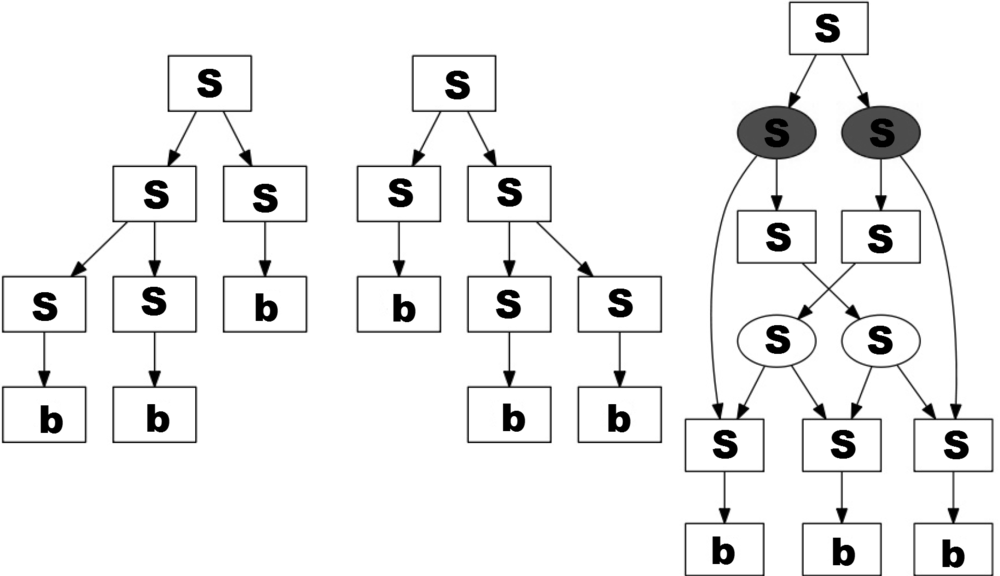
\includegraphics[width=\textwidth]{Gorokhov/courseworkpictures/SPPF.PNG}
\caption{Преобразование дерева разбора к SPPF}
\label{SPPF}
\end{figure}

\begin{figure}
$$
\begin{array}{crcl}
& \mbox{\texttt{ S }} &::=& \mbox{\texttt{ A B }} \& \mbox{\texttt{ D C}} \\
& \mbox{\texttt{ A }} & ::=& \mbox{\texttt{ a A |}}  \epsilon \\
& \mbox{\texttt{ B }} & ::=& \mbox{\texttt{ b B c |}}  \epsilon \\
& \mbox{\texttt{ C }} & ::=& \mbox{\texttt{ c C |}}  \epsilon \\
& \mbox{\texttt{ D }} & ::=& \mbox{\texttt{ a D b |}}\epsilon \\
\end{array}
$$
\caption{Грамматика для контекстно-зависимого языка \{$a^n b^n c^n, n \geq 0$\}}
\label{gabc}
\end{figure}

Алгоритм GLL позволяет работать с любыми КС-грамматиками, в том числе и сильно неоднозначными. Однако наличие сильной неоднозначности в грамматике сказывается на точности получаемых результатов и производительности. 
  Конъюнктивные грамматики при описании правил вывода используют операцию конъюнкции. Цепочка принадлежит языку, задаваемому такой грамматикой, если существует вывод по обоим конъюнктам. На рисунке~\ref{gabc} изображена грамматика для языка не являющегося контекстно-свободным, описанная с помощью операции конъюнкции. Такие грамматики дают возможность точно описать структуру тРНК, что позволяет снизить количество ошибок при разборе.

